\documentclass[11pt, a4paper]{article}

\usepackage[T1]{fontenc}
\usepackage[utf8]{inputenc}
\usepackage[french]{babel}
\usepackage{lmodern}
\usepackage{microtype}
\usepackage[top=2.0cm, bottom=2.2cm, left=1.8cm, right=1.8cm]{geometry}
\usepackage{booktabs}
\usepackage{float}
\usepackage[table]{xcolor}
\usepackage{hyperref}
\hypersetup{colorlinks=true, linkcolor=darkblue, citecolor=darkblue, urlcolor=darkblue}
\usepackage{graphicx}
\usepackage{titlesec}
\usepackage{fancyhdr}
\usepackage{parskip}
\usepackage{amsmath}
\usepackage{amssymb}
\usepackage{tikz}
\usetikzlibrary{arrows.meta, positioning}
\usepackage{caption}
\captionsetup{font=small, labelfont=bf}

\definecolor{darkblue}{RGB}{26, 60, 120}

\titleformat{\section}
  {\large\bfseries\color{darkblue}}
  {\thesection.}{0.6em}{}[\vspace{-4pt}\rule{\linewidth}{0.4pt}]

\titleformat{\subsection}
  {\normalsize\bfseries\color{darkblue}}
  {\thesubsection}{0.6em}{}

\pagestyle{fancy}
\fancyhf{}
\fancyhead[L]{\small\textcolor{gray}{TER -- Rapport mensuel}}
\fancyhead[R]{\small\textcolor{gray}{M1 MLDM -- UJM Saint-\'Etienne}}
\fancyfoot[C]{\small\thepage}
\renewcommand{\headrulewidth}{0.3pt}

\setcounter{secnumdepth}{2}

\begin{document}

\begin{titlepage}
    \centering
    \vspace*{1.5cm}
    {\large\color{darkblue}\textbf{Universit\'e Jean Monnet Saint-\'Etienne}}\\[0.3em]
    {\normalsize TER -- S2 2025/2026}

    \vspace{1.5cm}
    {\color{darkblue}\rule{\linewidth}{1.5pt}}
    \vspace{0.6cm}

    {\LARGE\bfseries\color{darkblue} Conception et \'evaluation d'un assistant juridique fond\'e sur l'IA,\\
    \'etude comparative entre RAG et fine-tuning}

    \vspace{0.4cm}
    {\large Rapport mensuel d'avancement -- juin/juillet 2026}
    \vspace{0.6cm}

    {\color{darkblue}\rule{\linewidth}{1.5pt}}
    \vspace{1cm}

    
\includegraphics[width=0.4\linewidth]{latex_assets/UJM-LOGO-NOIR.png}
    \vspace{1.5cm}

    {\large\bfseries Auteur}\\[0.8em]
    \begin{tabular}{c}
        {\large Chaabane Ouammou} \\[0.3em]
        \small M1 MLDM\\
    \end{tabular}

    \vspace{0.6cm}
    \begin{tabular}{c}
        {\normalsize Co-auteur : Bartosz Konior} \\[0.2em]
        \small M1 DSC\\
    \end{tabular}

    \vspace{1cm}
    \begin{tabular}{rl}
        \textbf{Encadrant :} & Marc Sebban \\[0.3em]
    \end{tabular}
\end{titlepage}

\pagecolor{white}
\color{black}
\setcounter{page}{1}
\twocolumn

\section{L'objet de ce mois de travail}

Le rapport pr\'ec\'edent laissait le projet avec une premi\`ere version fonctionnelle des deux pipelines et une seule comparaison entre eux, men\'ee sur un petit \'echantillon de questions. Ce mois a \'et\'e consacr\'e \`a reprendre presque chaque partie de cette premi\`ere version une par une, en v\'erifiant ce qui tenait toujours la route sous un examen plus attentif et ce qui ne tenait pas, et en construisant les \'el\'ements qui manquaient encore, en particulier une vraie comparaison statistique et une \'evaluation humaine. L'ordre ci-dessous suit \`a peu pr\`es l'ordre dans lequel le travail s'est r\'eellement d\'eroul\'e, en commen\c{c}ant par la recherche documentaire puisque tout le reste du pipeline RAG en d\'epend.

\section{Reprendre la recherche documentaire}

La recherche documentaire d\'ecide quels articles de loi le g\'en\'erateur voit jamais, donc avant de toucher \`a autre chose il semblait utile de v\'erifier \`a quel point elle \'etait vraiment bonne. Le mod\`ele d'embedding g\'en\'eraliste utilis\'e auparavant a \'et\'e remplac\'e par un mod\`ele multilingue plus large, \texttt{multilingual-e5-large}, et une base lexicale BM25 a \'et\'e ajout\'ee \`a c\^ot\'e, avec une combinaison hybride simple des deux classements. L'id\'ee \'etait de voir dans quelle mesure la recherche faible observ\'ee avant venait vraiment d'une limite du jeu de donn\'ees, et dans quelle mesure elle venait juste d'un mod\`ele d'embedding pas assez fort.

\begin{figure}[H]
\centering
\begin{tikzpicture}[
  box/.style={draw, rounded corners, minimum height=0.9cm, minimum width=2.9cm, align=center, font=\footnotesize, inner sep=4pt},
  arr/.style={-{Latex}, thick}
]
\node[box] (corpus) at (0,2.4) {Corpus d'articles};
\node[box] (embed)  at (0,0.8) {Embedding e5-large};
\node[box] (index)  at (0,-0.8) {Index vectoriel};
\node[box] (question) at (3.6,1.6) {Question};
\node[box] (retrieve) at (3.6,0) {Recherche top-$k$};
\node[box] (answer)   at (3.6,-1.6) {Mistral, r\'eponse};
\draw[arr] (corpus) -- (embed);
\draw[arr] (embed) -- (index);
\draw[arr] (index) -- (retrieve);
\draw[arr] (question) -- (retrieve);
\draw[arr] (retrieve) -- (answer);
\end{tikzpicture}
\caption{Pipeline de recherche documentaire. Le corpus est index\'e une fois, une question est compar\'ee \`a cet index au moment de la g\'en\'eration, et les articles retrouv\'es sont ajout\'es au prompt.}
\label{fig:ragdiagram}
\end{figure}

\begin{table}[H]
\centering
\small
\begin{tabular}{lccc}
\toprule
\textbf{M\'ethode} & \textbf{R@1} & \textbf{R@5} & \textbf{R@10} \\
\midrule
BM25 & 0.063 & 0.184 & 0.224 \\
mpnet (avant) & 0.021 & 0.074 & 0.097 \\
e5-large & 0.083 & 0.211 & 0.296 \\
Hybride BM25+e5 & 0.106 & 0.250 & 0.322 \\
\bottomrule
\end{tabular}
\caption{Qualit\'e de la recherche sur les 222 questions de test.}
\label{tab:retrieval}
\end{table}

Le changement aide clairement, le Recall@1 triple \`a peu pr\`es et la combinaison hybride fait encore un peu mieux sur chaque score, donc la recherche faible observ\'ee avant venait au moins en partie du choix du mod\`ele d'embedding plut\^ot que d'une limite dure du jeu de donn\'ees. M\^eme ainsi, le bon article manque encore plus de deux fois sur trois parmi les dix premiers r\'esultats, ce qui n'est pas un petit \'ecart et revient plus loin dans ce rapport.

Une chose m\'erite d'\^etre signal\'ee honn\^etement plut\^ot que pass\'ee sous silence. Le Recall@10 obtenu ici pour e5-large, 0.296, est nettement plus bas que ce qu'une \'evaluation ant\'erieure du m\^eme type de mod\`ele avait sugg\'er\'e. V\'erifier si des articles longs coup\'es trop t\^ot pouvait expliquer cela n'a pas donn\'e de r\'eponse convaincante, la plupart des articles sont courts. Deux autres explications restent possibles et n'ont pas encore \'et\'e test\'ees, que l'index pr\'ec\'edent ait pu inclure du texte suppl\'ementaire comme les intitul\'es de code et de chapitre, ou qu'il ait pu reposer sur un mod\`ele de recherche l\'eg\`erement ajust\'e sur le jeu de donn\'ees plut\^ot qu'utilis\'e tel quel. Ceci est laiss\'e ouvert plut\^ot que de choisir une explication sans l'avoir v\'erifi\'ee.

\section{\'Etendre les essais de fine-tuning}

Le r\'esultat de fine-tuning pr\'ec\'edent venait d'un seul essai, ce qui laissait ouverte la question de savoir combien de ce r\'esultat d\'ependait de la graine al\'eatoire particuli\`ere, ou de choix comme le rang de l'adaptateur ou la quantit\'e de donn\'ees d'entra\^inement utilis\'ee. Ce mois, avec un ensemble d'entra\^inement un peu plus grand disponible, cet essai unique a \'et\'e transform\'e en une petite famille d'essais qui changent un facteur \`a la fois.

Le fine-tuning fonctionne toujours en gelant le mod\`ele de base et en ajoutant un petit ajustement entra\^inable \`a quelques unes de ses matrices de poids plut\^ot qu'en r\'eentra\^inant tout le r\'eseau, ce qui est ce qui rend la proc\'edure possible sur un seul GPU grand public. Le rang de l'adaptateur, qui contr\^ole la taille de cet ajustement, est pass\'e de 16 \`a 32 ce mois, entra\^in\'e sur 580 questions au lieu de 380.

\begin{figure}[H]
\centering
\begin{tikzpicture}[
  box/.style={draw, rounded corners, minimum height=0.9cm, minimum width=3.1cm, align=center, font=\footnotesize, inner sep=4pt},
  arr/.style={-{Latex}, thick}
]
\node[box] (pairs)  at (0,1.4)  {Questions d'entra\^inement\\et r\'eponses de r\'ef\'erence};
\node[box] (lora)   at (0,-0.4) {Adaptateur sur\\Mistral gel\'e};
\node[box] (tuned)  at (3.9,0.5) {Mod\`ele fine-tun\'e};
\node[box] (answer) at (3.9,-1.3) {Question, r\'eponse};
\draw[arr] (pairs) -- (lora);
\draw[arr] (lora) -- (tuned);
\draw[arr] (tuned) -- (answer);
\end{tikzpicture}
\caption{Pipeline de fine-tuning. Seul le petit adaptateur est entra\^in\'e, les poids de base ne changent jamais, et aucune recherche documentaire n'intervient au moment de r\'epondre.}
\label{fig:ftdiagram}
\end{figure}

Un changement fait sp\'ecifiquement ce mois a \'et\'e l'ajout d'un petit ensemble de validation, 100 questions mises de c\^ot\'e avec une graine fixe, puisque l'essai pr\'ec\'edent n'avait aucun moyen de savoir si le mod\`ele apprenait vraiment \`a g\'en\'eraliser ou m\'emorisait simplement ses 380 exemples. Avec cet ensemble de validation en place, il est devenu possible de comparer le rang 16 au rang 32, l'attention seule \`a l'attention plus les couches de r\'eseau direct, et diff\'erentes quantit\'es de donn\'ees d'entra\^inement, sur un signal qui refl\`ete vraiment la g\'en\'eralisation plut\^ot que la seule perte d'entra\^inement.

\begin{table}[H]
\centering
\small
\begin{tabular}{lccc}
\toprule
\textbf{Variante} & \textbf{$n$} & \textbf{Perte train} & \textbf{Perte val.} \\
\midrule
principal (rang 32) & 580 & 0.834 & 0.679 \\
rang 8 & 580 & 0.850 & 0.710 \\
$n=380$ & 380 & 0.966 & 0.860 \\
$n=786$ & 786 & 0.736 & 0.561 \\
attn + MLP & 580 & 0.527 & 0.416 \\
\bottomrule
\end{tabular}
\caption{Variantes de fine-tuning s\'electionn\'ees, trois \'epoques chacune.}
\label{tab:finetune}
\end{table}

Plus de donn\'ees d'entra\^inement aide de fa\c{c}on assez r\'eguli\`ere, et laisser l'adaptateur toucher les couches de r\'eseau direct en plus de l'attention baisse beaucoup la perte de validation, m\^eme si l'\'ecart entre perte d'entra\^inement et perte de validation grandit aussi en m\^eme temps, ce qui signifie g\'en\'eralement que le mod\`ele colle plus \'etroitement \`a ses donn\'ees d'entra\^inement sans garantie que cela se transf\`ere bien \`a de nouvelles questions. La configuration principale a aussi \'et\'e r\'ep\'et\'ee sur trois graines al\'eatoires diff\'erentes, donnant une perte d'entra\^inement de $0.843 \pm 0.006$, assez stable en elle m\^eme, m\^eme si la section suivante montre que la qualit\'e des r\'eponses r\'eellement g\'en\'er\'ees varie plus \`a travers ces m\^emes trois graines que ce que la seule perte d'entra\^inement sugg\'ererait.

\section{Comparer quatre configurations correctement}

La comparaison pr\'ec\'edente utilisait trois configurations sur 50 questions et un seul essai. Ce mois une quatri\`eme configuration a \'et\'e ajout\'ee, le mod\`ele fine-tun\'e combin\'e \`a la recherche documentaire, pr\'ecis\'ement parce qu'il n'y avait aucun moyen de savoir avec le dispositif pr\'ec\'edent si les deux techniques aident sur la m\^eme faiblesse ou sur des faiblesses diff\'erentes, et la comparaison a \'et\'e d\'eplac\'ee vers les 222 questions de test compl\`etes avec un traitement statistique convenable plut\^ot qu'un seul chiffre par configuration.

Les intervalles de confiance ont \'et\'e obtenus en r\'e\'echantillonnant les 222 questions avec remise un grand nombre de fois et en regardant combien le score moyen bouge \`a travers ces r\'e\'echantillonnages, ce qui donne une id\'ee de combien un score donn\'e aurait pu plausiblement \^etre diff\'erent par le seul hasard. Chaque paire de configurations a aussi \'et\'e test\'ee deux fois pour v\'erifier une diff\'erence r\'eelle, une fois avec un test sur les diff\'erences r\'e\'echantillonn\'ees et une fois avec un test fond\'e sur les rangs qui fait moins d'hypoth\`eses sur les donn\'ees, et une correction a \'et\'e appliqu\'ee pour tenir compte du fait de tester six paires \`a la fois plut\^ot que chaque comparaison comme si elle \'etait la seule men\'ee.

\begin{table}[H]
\centering
\small
\begin{tabular}{lcc}
\toprule
\textbf{Config.} & \textbf{ROUGE-L} & \textbf{Intervalle 95\%} \\
\midrule
Zero-shot & 0.110 & 0.104 \`a 0.116 \\
RAG & 0.140 & 0.129 \`a 0.151 \\
Fine-tune & 0.147 & 0.136 \`a 0.160 \\
Fine-tune + RAG & 0.179 & 0.157 \`a 0.202 \\
\bottomrule
\end{tabular}
\caption{ROUGE-L avec intervalles de confiance bootstrap, jeu de test complet.}
\label{tab:generation}
\end{table}

\begin{figure}[H]
\centering

\includegraphics[width=\linewidth]{latex_assets/figs/config_comparison_ci.pdf}
\caption{ROUGE-L avec intervalles de confiance pour les quatre configurations.}
\label{fig:configci}
\end{figure}

Ajouter la recherche documentaire ou le fine-tuning seul bat clairement la base zero-shot dans les deux cas. La recherche documentaire et le fine-tuning pris s\'epar\'ement ne sont pas distinguables statistiquement l'un de l'autre, les deux tests s'accordent l\`a dessus, ce qui dit d\'ej\`a que les deux techniques sont plus proches en qualit\'e globale que leurs scores bruts dans le tableau ne le sugg\'ereraient \`a eux seuls. La comparaison entre le fine-tuning seul et la configuration combin\'ee est le seul cas o\`u les deux tests ne sont pas d'accord, donc cette comparaison pr\'ecise est trait\'ee ici comme non tranch\'ee plut\^ot que de choisir la r\'eponse qui para\^it la plus flatteuse.

Le r\'esultat de fine-tuning du rapport pr\'ec\'edent, mesur\'e sur 50 questions, \'etait nettement plus haut que le 0.147 mesur\'e ici sur les 222 questions compl\`etes, proche du bord sup\'erieur de l'intervalle de confiance dans le tableau~\ref{tab:generation} sans vraiment tomber dedans. Ceci n'est pas trait\'e comme une erreur \`a corriger, c'est une illustration assez directe de combien une estimation sur 50 questions peut bouger une fois mesur\'ee sur un ensemble de questions plus grand et plus repr\'esentatif, ce qui est la raison principale pour laquelle toute cette comparaison a \'et\'e refaite ce mois plut\^ot que r\'eutilis\'ee telle quelle.

\section{D'o\`u vient l'erreur restante}

Une fois la recherche documentaire et la g\'en\'eration toutes les deux plus solides, la question suivante naturelle \'etait laquelle des deux freinait encore le pipeline RAG. Une exp\'erience a \'et\'e mont\'ee pour r\'epondre \`a cela directement, les vrais articles pertinents ont \'et\'e plac\'es directement dans le prompt sans passer par le moteur de recherche du tout, ce qui retire compl\`etement l'erreur de recherche et montre ce que le g\'en\'erateur seul pourrait atteindre si la recherche \'etait parfaite.

\begin{table}[H]
\centering
\small
\begin{tabular}{lccc}
\toprule
\textbf{Condition} & \textbf{ROUGE-L} & \textbf{Exact match} & \textbf{Halluc.} \\
\midrule
Zero-shot & 0.110 & 0.005 & 0.144 \\
RAG (r\'eel) & 0.140 & 0.036 & 0.234 \\
Contexte oracle & 0.252 & 0.311 & 0.117 \\
\bottomrule
\end{tabular}
\caption{Exp\'erience de contexte oracle, mod\`ele de base dans tous les cas.}
\label{tab:oracle}
\end{table}

L'\'ecart entre la recherche r\'eelle et cette condition oracle est grand sur l'exactitude des citations, bien plus grand que l'\'ecart entre la recherche r\'eelle et l'absence totale de contexte, ce qui signifie que l'essentiel de ce qui manque actuellement vient de la recherche qui ne trouve pas le bon article plut\^ot que du mod\`ele qui \'echouerait \`a utiliser un bon article une fois qu'il l'a. Un r\'esultat n'\'etait pas attendu au d\'epart, le mod\`ele hallucine davantage avec la recherche r\'eelle qu'avec aucun contexte du tout, comme si un article plausible mais faux invitait \`a une invention plus confiante que de n'avoir rien du tout. Le m\^eme protocole a aussi \'et\'e lanc\'e une fois sur Qwen2.5-7B-Instruct \`a la place de Mistral, surtout pour v\'erifier que ce n'\'etait pas une particularit\'e d'un seul mod\`ele, et le m\^eme comportement est apparu l\`a aussi, la recherche documentaire am\'eliore la qualit\'e globale tout en doublant \`a peu pr\`es le taux d'hallucination.

La profondeur de recherche a aussi \'et\'e v\'erifi\'ee, puisque le pipeline utilisait cinq articles retrouv\'es de fa\c{c}on assez arbitraire. Essayer un, trois et dix articles sur un plus petit \'echantillon a montr\'e une qualit\'e maximale autour de trois, dix articles ne faisant pas mieux qu'un seul malgr\'e bien plus de texte, ce qui sugg\`ere qu'au del\`a d'un certain point le contexte suppl\'ementaire rend l'article pertinent plus difficile \`a rep\'erer plut\^ot que plus facile.

\section{Si le syst\`eme conna\^it ses propres limites}

Aucune des mesures ci-dessus ne dit rien sur une question \`a laquelle le syst\`eme devrait simplement refuser de r\'epondre. Un ensemble de 50 questions de ce type a \'et\'e construit ce mois, certaines sans aucun contenu juridique, certaines sur un syst\`eme juridique que BSARD ne couvre pas, et certaines faisant r\'ef\'erence \`a un article qui n'existe plus dans l'index, pour voir si l'une ou l'autre configuration reconna\^itrait cela plut\^ot que de r\'epondre quand m\^eme.

\begin{table}[H]
\centering
\small
\begin{tabular}{lc}
\toprule
\textbf{Config.} & \textbf{Abstention correcte} \\
\midrule
Zero-shot & 0.0\% \\
RAG & 2.0\% \\
\bottomrule
\end{tabular}
\caption{Abstention correcte sur 50 questions hors de port\'ee.}
\label{tab:abstention}
\end{table}

Le syst\`eme ne refuse presque jamais de r\'epondre. M\^eme pour une question qui n'a rien \`a voir avec le droit, il produit une r\'eponse \`a l'air confiant, num\'eros d'article invent\'es inclus, dans presque tous les cas. C'est l'une des faiblesses les plus nettes trouv\'ees ce mois et une de celles qu'aucune des deux techniques ne corrige d'elle m\^eme.

\section{Mesurer la qualit\'e sous deux angles}

Le recouvrement lexical avec un texte de r\'ef\'erence et le fait qu'une r\'eponse traite vraiment la question pos\'ee sont deux choses diff\'erentes, et il semblait pr\'ef\'erable de les mesurer s\'epar\'ement plut\^ot que de les fondre en un seul score. Une mesure d\'eterministe a \'et\'e ajout\'ee qui v\'erifie combien d'entit\'es nomm\'ees, de nombres et de d\'etails similaires dans la r\'eponse g\'en\'er\'ee apparaissent aussi dans le texte de r\'ef\'erence, donnant une id\'ee de l'ancrage factuel sans avoir besoin d'un autre mod\`ele pour en juger\footnote{Cette s\'eparation entre une mesure d'ancrage d\'eterministe et un juge ind\'ependant pour ce qui est vraiment subjectif suit l'approche utilis\'ee par Bouvard, Ciancone, Gourru et Schaeffer pour une comparaison similaire entre RAG et fine-tuning (APIA 2024), r\'eimpl\'ement\'ee ici plut\^ot que r\'eutilis\'ee directement.}. S\'epar\'ement, un mod\`ele de langage ind\'ependant, Phi-3.5-mini-instruct, a \'et\'e utilis\'e pour juger si chaque r\'eponse traite bien ce qui \'etait vraiment demand\'e, en notant chaque r\'eponse plusieurs fois plut\^ot qu'une seule puisqu'un seul jugement d'un mod\`ele de langage n'est pas tr\`es stable.

\begin{table}[H]
\centering
\small
\begin{tabular}{lcc}
\toprule
\textbf{Config.} & \textbf{Fid\'elit\'e} & \textbf{Pertinence /5} \\
\midrule
Zero-shot & 0.054 & 5.00 \\
RAG & 0.295 & 4.85 \\
Fine-tune & 0.298 & 4.73 \\
Fine-tune + RAG & 0.324 & 4.62 \\
\bottomrule
\end{tabular}
\caption{Fid\'elit\'e au texte de r\'ef\'erence et pertinence jug\'ee.}
\label{tab:fidjudge}
\end{table}

Le score moyen de pertinence reste haut et presque plat \`a travers les configurations, mais regarder la distribution compl\`ete plut\^ot que la seule moyenne montre une part petite mais qui grandit r\'eguli\`erement de r\'eponses jug\'ees clairement hors sujet en allant du zero-shot vers la configuration combin\'ee. Lu avec la lecture qualitative d'une section plus loin, cela sugg\`ere que la recherche documentaire et le fine-tuning \'eloignent parfois la r\'eponse de la question r\'eellement pos\'ee, un effet r\'eel mais plus petit que l'\'ecart d'ancrage des citations d\'ecrit plus haut.

\section{Ce qui rend une question difficile}

Deux explications possibles pour lesquelles certaines questions obtiennent de meilleures r\'eponses que d'autres ont \'et\'e v\'erifi\'ees directement plut\^ot que suppos\'ees, la longueur de la question et le nombre d'articles de loi vraiment n\'ecessaires pour y r\'epondre. La longueur de la question s'est av\'er\'ee n'avoir presque aucun lien avec la qualit\'e de la r\'eponse. Le nombre d'articles n\'ecessaires, en revanche, corr\`ele clairement et de fa\c{c}on constante avec une qualit\'e plus basse dans chaque configuration, donc la longueur \'etait la mauvaise chose \`a supposer importante et le vrai facteur est combien de r\`egles s\'epar\'ees doivent \^etre combin\'ees dans une seule r\'eponse.

\begin{figure}[H]
\centering
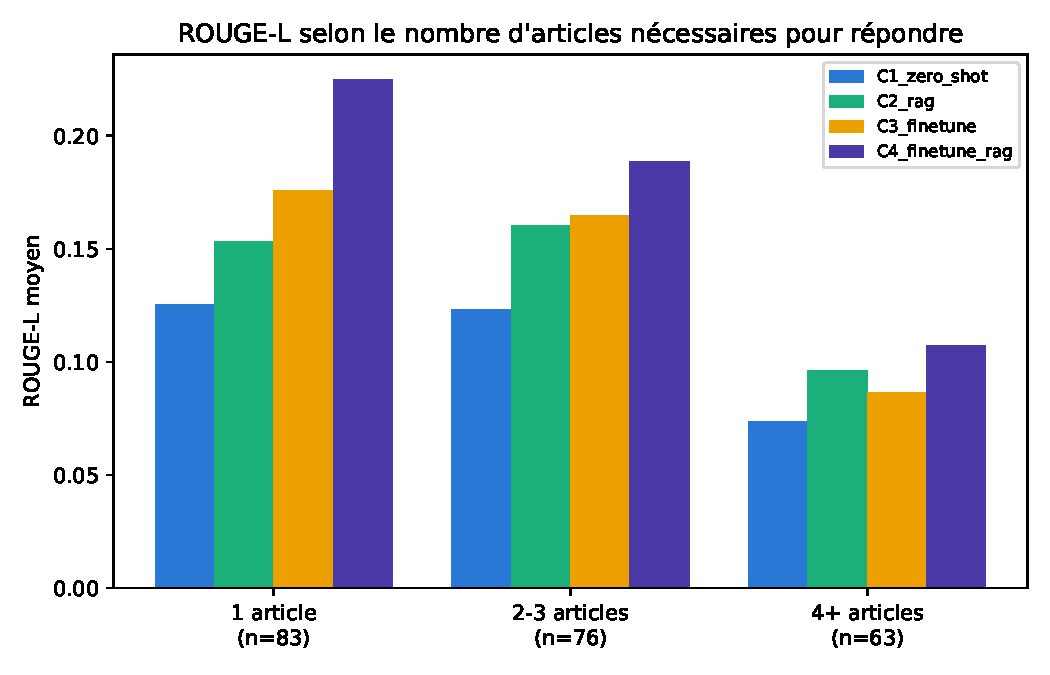
\includegraphics[width=\linewidth]{latex_assets/figs/difficulty_bucket_rouge.pdf}
\caption{ROUGE-L regroup\'e par nombre d'articles requis.}
\label{fig:difficulty}
\end{figure}

La qualit\'e reste globalement stable pour les questions n\'ecessitant un \`a trois articles et chute nettement d\`es que quatre ou plus sont n\'ecessaires, dans chaque configuration sans exception, et ni la recherche documentaire ni le fine-tuning ne corrige cela d'eux m\^emes. Un classifieur simple a aussi \'et\'e entra\^in\'e pour pr\'edire, avant m\^eme la g\'en\'eration, si une question donn\'ee a des chances d'obtenir une r\'eponse correctement cit\'ee, en utilisant seulement des informations disponibles \`a l'avance comme la longueur de la question et sa cat\'egorie. Il s\'epare les questions fiables des questions peu fiables nettement mieux que le hasard, et les m\^emes variables qui portent cette pr\'ediction, surtout la longueur de la question et la fr\'equence de sa cat\'egorie dans les donn\'ees d'entra\^inement, pointent vers la m\^eme conclusion, que certaines questions sont pr\'evisiblement plus dures avant m\^eme que le mod\`ele ne g\'en\`ere quoi que ce soit.

\section{Un adaptateur sp\'ecialiste d'un domaine}

Regarder les r\'esultats d\'ecoup\'es par cat\'egorie juridique sugg\'erait une question naturelle, un adaptateur entra\^in\'e sur un seul domaine ferait il mieux sur ce domaine qu'un adaptateur g\'en\'eraliste. Un adaptateur sp\'ecialiste a \'et\'e entra\^in\'e sur le sous-ensemble des questions d'entra\^inement concernant le Code Civil, avec moins d'exemples que l'adaptateur g\'en\'eraliste puisque ce sous-ensemble est plus petit, et compar\'e au g\'en\'eraliste sur les m\^emes questions de test.

Le r\'esultat est ressorti mitig\'e plut\^ot que comme une victoire nette pour la sp\'ecialisation. Sur son propre domaine le sp\'ecialiste est l\'eg\`erement meilleur en recouvrement lexical mais hallucine nettement plus, et combin\'e \`a la recherche documentaire il fait moins bien que le g\'en\'eraliste dans les deux domaines tout en hallucinant moins dans les deux. Comme le sp\'ecialiste a \'et\'e entra\^in\'e sur moins d'exemples que le g\'en\'eraliste, cette comparaison m\'elange l'effet de restreindre le domaine avec l'effet d'avoir simplement moins de donn\'ees d'entra\^inement, et les r\'esultats de fine-tuning plus haut dans ce rapport montrent d\'ej\`a que moins d'exemples \`a eux seuls font baisser la qualit\'e. Cette exp\'erience ne tranche pas vraiment si la sp\'ecialisation par domaine aide, elle montre surtout qu'un test \'equitable de cette id\'ee demande des tailles d'entra\^inement comparables, ce qui est pr\'evu comme prochaine \'etape.

\section{Confronter les r\'esultats au jugement humain}

Toute mesure jusqu'ici est automatique, et un score automatique peut \^etre coh\'erent avec lui m\^eme tout en ne correspondant pas \`a ce qu'une personne pr\'ef\'ererait vraiment lire. Les deux auteurs, avec un troisi\`eme annotateur dont la collecte de donn\'ees est encore en cours, ont compar\'e \`a l'aveugle la configuration avec recherche documentaire et la configuration fine-tun\'ee sur 60 questions, sans savoir quel c\^ot\'e \'etait lequel.

\begin{table}[H]
\centering
\small
\begin{tabular}{lcc}
\toprule
\textbf{Annotateur} & \textbf{Pr\'ef\`ere RAG} & \textbf{Pr\'ef\`ere fine-tune} \\
\midrule
Annotateur 1 & 70.0\% & 10.0\% \\
Annotateur 2 & 55.0\% & 8.3\% \\
\bottomrule
\end{tabular}
\caption{Pr\'ef\'erence par paire \`a l'aveugle, 60 questions communes.}
\label{tab:arena}
\end{table}

L'accord entre les deux annotateurs sur les questions communes \'etait mod\'er\'e plut\^ot que fort, ce qui est rapport\'e honn\^etement plut\^ot que suppos\'e acquis, et discut\'e un peu plus loin. M\^eme ainsi, les deux annotateurs ont pr\'ef\'er\'e clairement et ind\'ependamment la configuration avec recherche documentaire \`a la configuration fine-tun\'ee, par une marge large. Ceci est en tension r\'eelle avec la comparaison automatique pr\'ec\'edente sur 50 questions, qui avait plac\'e le mod\`ele fine-tun\'e devant sur le recouvrement lexical. Plut\^ot que d'essayer d'expliquer cette tension, elle est prise ici comme le signe le plus clair ce mois qu'une comparaison lexicale sur petit \'echantillon et un jugement humain \`a l'aveugle sur les deux m\^emes syst\`emes ne vont pas toujours dans le m\^eme sens, ce qui est la raison pour laquelle les deux sont maintenant mesur\'es c\^ote \`a c\^ote.

\section{Ce que la lecture des r\'eponses a montr\'e}

Au del\`a des chiffres, lire directement les r\'eponses annot\'ees a fait ressortir quelques sch\'emas qui m\'eritent d'\^etre d\'ecrits avec leurs propres mots. L'erreur la plus courante est une inversion de r\^oles juridiques, une obligation attribu\'ee \`a la mauvaise partie, souvent sur des paires de questions qui ne diff\`erent que d'un mot, mari\'e contre cohabitant l\'egal par exemple, o\`u le bon article diff\`ere d'une fa\c{c}on subtile facile \`a manquer aussi bien pour la recherche que pour la g\'en\'eration. Du texte de loi invent\'e appara\^it aussi assez souvent, et \'etant donn\'e que l'hallucination ne dispara\^it pas compl\`etement m\^eme sous la condition de contexte oracle, une partie au moins de cela semble \^etre une tendance g\'en\'erale du mod\`ele de base plut\^ot que purement une cons\'equence d'une mauvaise recherche. Un nombre plus petit de r\'eponses d\'erive simplement loin de la question pos\'ee, g\'en\'eralement quand un passage retrouv\'e est proche du sujet sans vraiment r\'epondre \`a ce qui \'etait demand\'e. Un dernier sch\'ema, du texte r\'ep\'et\'e ou coup\'e dans certaines r\'eponses, ressemble \`a un probl\`eme de r\'eglage du d\'ecodage plut\^ot qu'\`a une limite du mod\`ele, puisque la g\'en\'eration n'utilise actuellement aucune p\'enalit\'e de r\'ep\'etition, et corriger cela est une t\^ache petite et concr\`ete pour le mois prochain plut\^ot qu'une question de recherche ouverte.

Une limite soulev\'ee par les annotateurs eux m\^emes m\'erite d'\^etre dite clairement, aucun des deux n'est un professionnel du droit form\'e, et distinguer une affirmation juridique subtilement fausse d'une affirmation correcte peut \^etre vraiment difficile \`a v\'erifier \`a partir du contexte raccourci montr\'e pendant l'annotation. C'est une vraie limite de l'\'evaluation humaine telle qu'elle est, pas quelque chose \`a cacher, et c'est en partie pourquoi l'accord mod\'er\'e entre annotateurs ci-dessus ne devrait pas \^etre lu comme de la n\'egligence.

\section{Difficult\'es pratiques ce mois}

Comme dans le rapport pr\'ec\'edent, les probl\`emes techniques les plus longs \`a r\'esoudre sont list\'es ici bri\`evement plut\^ot que sous forme de r\'ecit. Les identifiants d'articles de loi du jeu de donn\'ees se sont av\'er\'es ne pas \^etre uniform\'ement num\'eriques, une part significative suit des formats r\'egionaux et une part plus petite porte un artefact laiss\'e par la mani\`ere dont les donn\'ees ont \'et\'e collect\'ees \`a l'origine, les deux devant \^etre nettoy\'es avant qu'une m\'etrique fond\'ee sur les citations puisse \^etre fiable. Aucun ensemble de validation n'existait pour le fine-tuning avant ce mois, ce qui rendait impossible de distinguer un mod\`ele qui g\'en\'eralise d'un mod\`ele qui m\'emorise sur quelques centaines d'exemples, et un petit ensemble de validation fixe a \'et\'e ajout\'e sp\'ecifiquement pour combler ce manque. Comme chaque calcul ce mois tourne comme un script ind\'ependant plut\^ot que de partager du code, un correctif appliqu\'e \`a un endroit, le plus souvent sauvegarder les r\'esultats interm\'ediaires apr\`es chaque \'etape d'un long calcul plut\^ot que seulement \`a la fin, ne se propageait pas automatiquement aux autres et devait \^etre r\'eappliqu\'e \`a la main. Enfin, le quota de GPU gratuit utilis\'e pour ces exp\'eriences n'autorise que deux calculs en m\^eme temps, et relancer un calcul apr\`es un correctif n'arr\^ete pas automatiquement l'ancienne version encore en cours, ce qui a caus\'e plus d'un retard \'evitable avant que cela ne soit compris.

\section{Ce qui reste avant le rapport final}

Trois \'el\'ements se reportent directement sur la suite. L'\'ecart de recherche documentaire d\'ecrit au d\'ebut de ce rapport doit \^etre r\'esolu ou au moins r\'eduit. La collecte de donn\'ees du troisi\`eme annotateur et une lecture plus formelle et doublement annot\'ee des erreurs, seulement esquiss\'ee qualitativement ici, doivent \^etre termin\'ees. La g\'en\'eration devrait aussi \^etre relanc\'ee avec une p\'enalit\'e de r\'ep\'etition ajout\'ee, pour v\'erifier combien du probl\`eme de texte r\'ep\'et\'e ou coup\'e d\'ecrit plus haut est simplement un r\'eglage \`a corriger plut\^ot qu'une vraie limite des mod\`eles et des donn\'ees actuels.

\begin{thebibliography}{9}

\bibitem{hu2022lora}
E. J. Hu et al.
\textit{LoRA: Low-Rank Adaptation of Large Language Models.}
ICLR 2022. arXiv:2106.09685.

\bibitem{dettmers2023qlora}
T. Dettmers et al.
\textit{QLoRA: Efficient Finetuning of Quantized LLMs.}
NeurIPS 2023. arXiv:2305.14314.

\bibitem{lewis2020rag}
P. Lewis et al.
\textit{Retrieval-Augmented Generation for Knowledge-Intensive NLP Tasks.}
NeurIPS 2020. arXiv:2005.11401.

\bibitem{bouvard2024derby}
C. Bouvard, M. Ciancone, A. Gourru, M. Schaeffer.
\textit{Derby LLM : \'Evaluation comparative des approches RAG et fine-tuning.}
APIA 2024. hal-04638460.

\bibitem{louis2021bsard}
A. Louis, G. Spanakis.
\textit{A Statutory Article Retrieval Dataset in French.}
ACL 2021. arXiv:2108.11792.

\bibitem{zhang2020bertscore}
T. Zhang, V. Kishore, F. Wu, K. Q. Weinberger, Y. Artzi.
\textit{BERTScore: Evaluating Text Generation with BERT.}
ICLR 2020. arXiv:1904.09675.

\bibitem{ovadia2023finetune}
O. Ovadia, M. Brief, M. Mishaeli, O. Elisha.
\textit{Fine-Tuning or Retrieval? Comparing Knowledge Injection in LLMs.}
arXiv:2312.05934, 2023.

\end{thebibliography}

\end{document}
